\chapter{The Wave Function}

\section{One Dimensional Systems}

Up until now we've dealt exclusively with \emph{discrete} system like spin.  In these cases, we used column vectors to represent the quantum state of our particle; for example, for spin-1/2, we had
\[
\ket{\psi} \to \begin{pmatrix} \braket{+}{\psi} \\ \braket{-}{\psi} \end{pmatrix}.
\]
Take careful note of the notation; each element in the column vector is a matrix element, and you can clearly see the basis $\ket{+},\ket{-}$ used.  In general, we would have a system that has $n$ elements, where $n$ could be three (say, for spin-1) or more -- all the way up to infinity:
\[
\ket{\psi} \to \begin{pmatrix} \braket{a_1}{\psi} \\ \braket{a_2}{\psi} \\ \braket{a_3}{\psi} \\ \vdots \end{pmatrix}.
\]
All of the quantum mechanical rules that we've discussed are identical regardless of the number of possible states of the system.

Now, though, it's time for something a little different (don't worry, only a little).  We want to work in the \emph{position representation}, in which case we might write our state as the column vector
\begin{equation}
\label{eq_pos_col_vec}
\ket{\psi} \to \begin{pmatrix} \braket{x_1}{\psi} \\ \braket{x_2}{\psi} \\ \braket{x_3}{\psi} \\ \vdots \end{pmatrix},
\end{equation}
where the kets $\ket{x_i}$ are the position eigenstates.  There's one problem here, though: not only are there an infinite number of position states, they are \emph{continuous} -- in general our particle could be at position $x=1.0$, or $x =1.01$, or $x = 1.000001$.  In the language of linear algebra, we say that the spectrum of eigenvalues is continuous.  

It's difficult to use a column vector to represent our state in the position basis -- it's really more suited to discrete systems.  But it's pretty easy to imagine how to extend the idea: each element in equation (\ref{eq_pos_col_vec}) is the state ``evaluated'' at the position $x_i$, and if these positions run continuously, what we really have is a \emph{function}:
\begin{equation}
\label{eq_wave_function_defined}
\boxed{
\ket{\psi} \to  \psi(x) \quad \text{where} \quad \psi(x) \equiv \braket{x}{\psi}.
}
\end{equation}

We already know that we can represent a quantum state as a ket, or a column vector, and now we can also use a function.  But what exactly does the function $\psi(x)$ mean?  Well, remember that the inner product $\braket{x}{\psi}$ is the probability \emph{amplitude} (we have to square it to get the actual probability) of the quantum state to be measured in the position eigenstate $\ket{x}$.  That means the probability of finding a particle to be at position $x$ is
\[
\mathcal{P}(x) = | \braket{x}{\psi}|^2 = \braket{\psi}{x}\braket{x}{\psi} = \psi^*(x)\psi(x) = |\psi(x)|^2.
\]
Actually, that's not quite correct; our jump to continuous systems means that $\mathcal{P}(x)$ is actually a probability \emph{density}, and we properly have to say that $\mathcal{P}(x)dx$ is the probability of finding the particle between the position $x$ and $x + dx$.  If we want to know about a finite region, we'd have to integrate:
\begin{equation}
\boxed{
\int_a^b \mathcal{P}(x) dx = \int_a^b |\psi(x)|^2 dx \quad  \text{ \parbox[l]{1.8in}{is the probability of finding the particle between $x = a$ and $x=b$.}} 
}
\end{equation}

Like all quantum states we've discussed so far, states written in the position representation must be too; here, that means
\begin{equation}
\braket{\psi}{\psi} = 1 \quad \to \quad \int_{-\infty}^\infty |\psi(x)|^2 dx = 1. 
\end{equation}
In words, that means we have to find the particle \emph{somewhere} with 100\% probability.

The structure of the inner product above carries over to \emph{all} inner products, so in general we'll calculate the inner product between state $\ket{\phi}$ and state $\ket{\psi}$ in position space as
\begin{equation}
\braket{\phi}{\psi} \to \int_{-\infty}^\infty \phi^*(x) \psi(x) dx. 
\end{equation}
That means we can calculate probabilities in position space, too, with
\begin{equation}
\mathcal{P}_{\psi \to \phi} = |\braket{\phi}{\psi}|^2 \to \left| \int_{-\infty}^\infty \phi^*(x) \psi(x) dx \right|^2
\end{equation}
being the probability of measuring the state $\ket{\phi}$ to be in the state $\ket{\phi}$.

What about expectation values?  For that, we'll need to write the operator in position space as well:
\[
\hat{A} \to A(x)
\]
(as we'll see, operators in position space can take the form of functions of $x$ or derivatives with respect to $x$).  Then the expectation value carries over naturally to become
\begin{equation}
\avg{A} = \bra{\psi} \hat{A} \ket{\psi} \to  \int_{-\infty}^\infty \psi^*(x) A(x) \psi(x) dx.
\end{equation}
For example, the expectation value of position itself, a quantity we'll be calculating frequently, is
\begin{equation}
\avg{x} = \bra{\psi} \hat{x} \ket{\psi} \to  \int_{-\infty}^\infty \psi^*(x) x \psi(x) dx = \int_{-\infty}^\infty x |\psi|^2 dx.
\end{equation}


\section{Position Indeterminacy} 

We've already talked about indeterminacy -- the idea that some observables simply don't have definite values in some quantum states -- back when we talked about measuring spin in Section \ref{sec_indeterminant_states}.  But the issue hits a little differently when we add \emph{position} into the mix -- after all, position is something we readily understand on an everyday basis, whereas spin is some weird quantum thing.

Consider a particle described by the wave function $\psi(x)$ as shown in Figure \ref{fig_example_wave_function}.  Even at a quick glance the wave function tells us quite a bit about where we would be likely to find the particle -- more likely at position A, for example, and not at all at position B. Of course, like with spin, we can't say exactly where the particle is located \emph{before} we measure its position -- it's indeterminant.  It doesn't just have an \emph{unknown} position -- it doesn't have a position at all.

\begin{figure}
\centering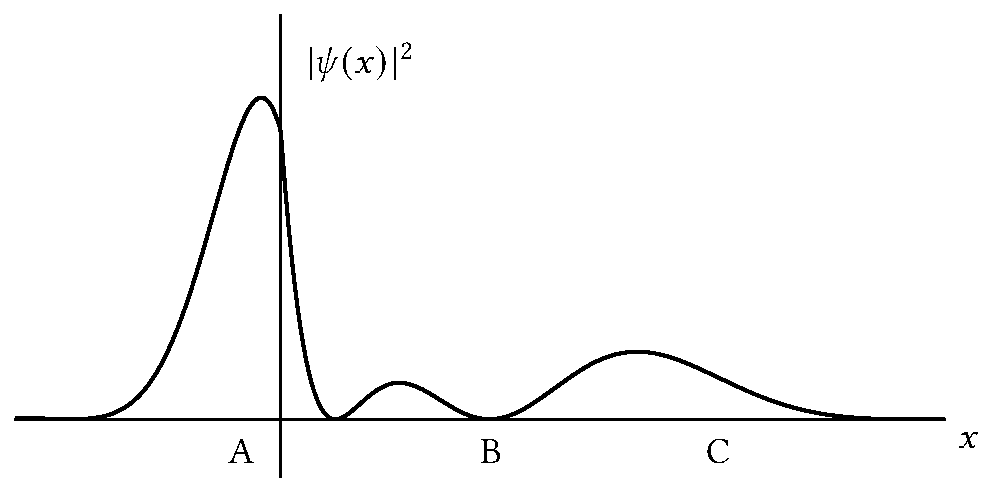
\includegraphics[width=0.8\linewidth]{Figures/Chapter 8/fig_example_wave_function.pdf}
\caption{An example wave function.}
\label{fig_example_wave_function}
\end{figure}

To see this more clearly, suppose we go ahead and measure the position of our particle, and suppose that it happens to be found at position C.  Once we make that measurement, the wave function will change -- as with measuring spin, it will ``collapse'' to the eigenstate corresponding to the measurement we made.  In this case that's a high, sharp spike at position C, as shown in Figure \ref{fig_collapsed_wave_function}.  Technically this is a Dirac delta function, as we'll discuss later, but it makes sense -- subsequent measurements will keep returning position C, at least as long as they're made relatively quickly after the first and before the wave function evolves in time (which it will do according to the Schr\"odinger equation).

\begin{figure}
\centering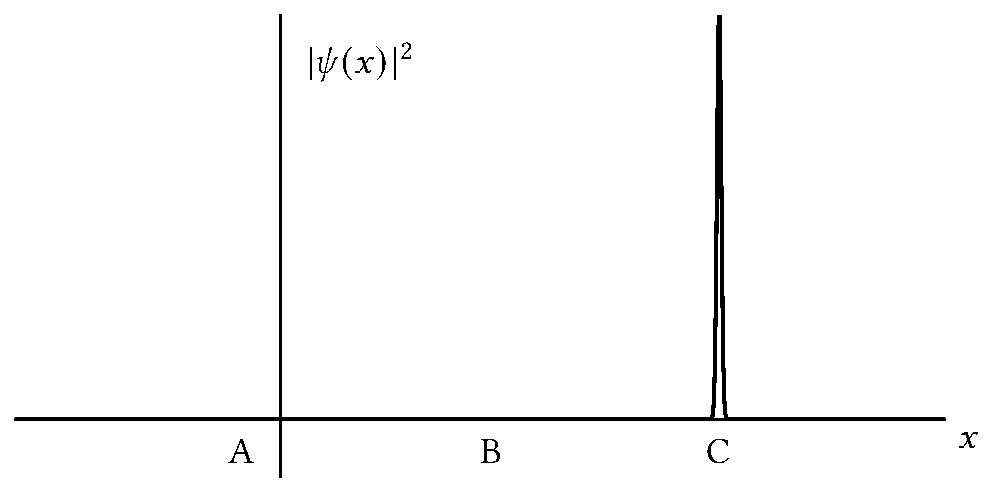
\includegraphics[width=0.8\linewidth]{Figures/Chapter 8/fig_collapsed_wave_function.pdf}
\caption{The wave function has collapsed to a spike at point C.}
\label{fig_collapsed_wave_function}
\end{figure}

But then the question is -- where was the particle \emph{just before} its position was measured?  The options here are the same as back in Section \ref{sec_indeterminant_states}: we could take a \emph{realist} position (the particle was at position C), hold to the \emph{Copenhagen interpretation} (the particle didn't have a position at all), or give up and refuse to answer.  As before, we'll go with the standard Copenhagen interpretation, which says that the position of the particle was indeterminant -- it somehow didn't have a position at all, and somehow measuring the particle caused it to ``take a stand'' and pick a position value consistent with the wave function of the particle.  To say this is out of our normal range of experience is an understatement, but it seems to be how the universe works.  The act of measurement in quantum mechanics is still a hotly debated and studied phenomenon among physicists.

\section{The Energy Eigenvalue Equation}

So, why are we talking about position all of sudden?  Up to now we haven't had to worry about it -- we discussed spin, or neutrino flavours, but haven't yet had to worry about \emph{where} a particle is.  But as you learned in your classical mechanics course, potential energy can depend on position, and, in one dimension, the total energy will be
\[
E = T + V = \frac{p_x^2}{2m} + V(x),
\]
where the first term is of course the kinetic energy (which depends on momentum) and the second is potential energy (which depends on position).  In fact \emph{any} dynamical variable can always be written in terms of momentum and position.

We should probably figure out how to deal with position and momentum in quantum mechanics, then.  These are both \emph{observables}, so to ``turn on'' quantum mechanics, we make them \emph{operators}.

I'll start with position, which is a little easier to understand right away:  the observable position $x$ is represented by an operator $\hat{x}$.  In the position representation, the operator just takes the form of $x$:
\begin{equation}
\hat{x} \to x.
\end{equation}
That is, the actual operation is \emph{multiply the state by the variable $x$}.  This will all make sense when we use the operator, even if it sounds a little confusing now.

For the observable momentum $p_x$, the quantum operator is $\hat{p}_x$, and in the position representation
\begin{equation}
\hat{p}_x \to -i\hbar \frac{d}{dx}.
\end{equation}
Somehow, the momentum operation is to take the derivative of the state and multiply by $-i\hbar$.  These two observables are summarized in Table \ref{tab_x_and_p}.  And if you're wondering why the momentum operator is a spatial derivative, don't worry, we'll dig deeper into $\hat{p}$ later.

\begin{table}
\centering
\begin{tabular}{c c c m{1in}}
Observable & Operator & Position Representation & Operation \\
\hline
$x$ & $\hat{x}$ & $x$ & Multiply by $x$ \\[3pt]
$p_x$ & $\hat{p}_x$ & $-i\hbar \frac{d}{dx}$ & Take the derivative and multiply by $-i\hbar$ \\
\hline
\end{tabular}
\caption{The position and momentum observables in the position representation.}
\label{tab_x_and_p}
\end{table}

The Hamiltonian operator for a particle in one-dimensional motion along the $x$-axis can now be written down in position space as
\begin{equation}
\boxed{
\hat{H} = \frac{\hat{p}_x^2}{2m} + V(\hat{x}) \to -\frac{\hbar^2}{2m} \frac{d^2}{dx^2} + V(x).
}
\end{equation}
We normally write the energy eigenvalue equation as
\[
\hat{H} \ket{E_n} = E_n \ket{E_n},
\]
but in the position representation we'll use a different letter $\phi$ to denote the energy eigenstate:
\[
\ket{E_n} \to \phi_n(x).
\]

The energy eigenvalue equation then becomes
\begin{equation}
\boxed{
-\frac{\hbar^2}{2m} \frac{d^2 \phi_n}{dx^2} + V(x)\phi_n(x) = E_n \phi_n(x).
}
\end{equation}
This equation is often called the \emph{time-independent Schr\"odinger equation}, although I'll keep calling it the energy eigenvalue equation.  Notice that in position space we've gone from solving simple matrix equations to now solving differential equations.


\section{Bound and Unbound States}

%
%
%

\section*{Problems}
\addcontentsline{toc}{section}{Problems}
\markright{Problems}%

\begin{problem}[Some problems]
\label{prob_some}

Test

\end{problem}
